\chapter{WebAssembly}

Míg a megelőző fejezetek a dolgozat eredményét jelentő könyvtár kriptográfiai alapjait fektették le, addig ebben a fejezetben az implementációhoz használt egyik legfontosabb technológiát, a WebAssemblyt (röviden: Wasm) mutatjuk be részletesen. 

Annak érdekében, hogy érezhető legyen a WebAssembly valódi jelentősége, ismertetésre kerülnek a hasonló célokat szolgáló, azonban ma már túlhaladottnak tekinthető eszközök. Ezt követően a WebAssembly áttekintését adjuk, kiemelt figyelmet szentelve azoknak az előnyös tulajdonságoknak, melyek megkülönböztetik a korábbi technológiáktól. Végül egy rövid példa zárja a fejezetet, ízelítőt adva a fejlesztési folyamatból.

\section{Előzmények}

A dinamikus weboldalak létrehozását lehetővé tevő JavaScript programozási nyelv 1995-ben jelent meg először a Netscape Navigator 2.0 böngészőben \cite{JavaScriptAnnouncement}. Bár szerveroldali alkalmazása már a kezdetektől is lehetséges volt, azonban a 2010-es évekig (a Node.js feltűnéséig) inkább a kliensoldalon játszott meghatározó szerepet, hiszen az első pillanattól kezdve támogatta a HTML oldalak manipulációját, miközben egyszerű, laikusok számára is érthető szintaxissal bírt.

Ugyanakkor nem a JavaScript az egyetlen olyan technológia, mely az elmúlt évtizedekben a dinamikus webes tartalmak elkészítését, vagy egyszerűen csak a böngészőben való, lehetőleg hatékony kódfuttatás elősegítését szolgálta. A teljesség igénye nélkül érdemes megemlékezni a következő technológiákról, melyek mindegyike ilyen, vagy olyan szempontból, de az előbbi célokra készült, így egyúttal a WebAssembly előzményének is tekinthető:

\begin{itemize}
    \item
    Java Applet,

    \item
    Adobe Flash,

    \item
    ActiveX,

    \item
    Native Client (NaCl), illetve Portable Native Client (PNaCl),

    \item
    asm.js.
\end{itemize}

A következőkben e technológiák főbb jellemzőit tekintjük át: az előbbi három esetében csak érintőlegesen, míg a (P)NaCl és az asm.js esetében részletesebben.

\subsection{Korai beépülő modulok}

A Java programozási nyelvhez kapcsolódó platformfüggetlen infrastruktúrát használják ki az \textit{appletek}, melyek más alkalmazásokba beágyazható kis programok\cite{JavaDocs::java.applet.Applet}. Az egyik legnépszerűbb beágyazó környezetet a webböngészők jelentik, melyek beépülő modulok segítségével képesek az \textit{appletek} megjelenítésére \cite{JavaPlugInTechnology}. Természetesen az \textit{appletek} forráskódja a beágyazó böngészőtől teljesen független. Kiemelendő, hogy az \textit{appletek} alapértelmezés szerint egy zárt, úgynevezett \textit{sandbox} környezetben futnak, mely megakadályozza, hogy kártékony tevékenységeket hajtsanak végre a felhasználó tudta nélkül \cite{TheJavaTutorials::JavaApplets}.

A Flash először csak gyors rajzolási és animációs képességekkel kívánta felruházni a böngészőket, az évek során azonban egy átfogó multimédia platformmá fejlődött \cite{Gay::TheHistoryOfFlash}. Létrejöttében kulcsszerepet játszott az \textit{appletek} multimédiás célokra történő alkalmatlansága. A Flash animációk böngészőben történő megjelenítéséhez szintén egy beépülő modul szükséges, ez a Flash Player \cite{AdobeFlashPlayer}.

Említésre méltó a Microsofthoz köthető ActiveX Technologies keretrendszer, mely úgynevezett ActiveX Controlok útján tette lehetővé dinamikus komponensek és objektumok beágyazását a HTML oldalakba \cite{MicrosoftAnnouncesActiveXTechnologies}. Habár az ActiveX Controlok is egy beépülő böngésző modult igényelnek a megfelelő működéshez, azonban a technológia jelentősen eltér az előzőleg látottaktól. Egyfelől az egyes komponensek platformfüggő binárisok formájában kerülnek terjesztésre \cite{Grimes::MaliciousMobileCode}, másfelől azok közvetlenül kerülnek lefuttatásra, így tetszőleges műveleteket végrehajthatnak a felhasználó számítógépén \cite{DesigningSecureActiveXControls}.

Ma már ezen három technológia mindegyike túlhaladottnak tekinthető. Az Applet API a Java 9-ben már \textit{deprecated} annotációval bír \cite{JEP289::DeprecateTheAppletAPI}, a Flash támogatását az Adobe 2020-ban végleg beszünteti \cite{FlashAndTheFutureOfInteractiveContent}, az ActiveX pedig az úgynevezett \textit{evergreen} böngészők egyikében sem támogatott már, még a Microsoft Edge-ben sem \cite{ABreakFromThePast}.

\subsection{Native Client, Portable Native Client}

Míg az előzőleg felsorolt technológiák inkább a böngésző, mint alkalmazásfejlesztési platform hiányosságait kívánták pótolni, addig a Google ernyője alatt megszülető Native Client (röviden NaCl) a teljesítményre fókuszál. A NaCl a natív (azaz például C vagy C++ nyelven írt) programok hatékony futtatását tette lehetővé a böngésző által biztosított \textit{sandbox} környezetben \cite{Yee::NativeClient}. A NaCl platformfüggetlen testvére a Portable Native Client (röviden PNaCl), mely a HTML oldalakba való beágyazást is biztosítja \cite{NativeClient::NaClAndPNaCl}.

A PNaCl modulokat (\textit{pexe}) egy LLVM-alapú fordító segítségével lehet előállítani. Érdekesség, hogy az így elkészült modul a fordító belső, átmeneti reprezentációját használja, a tartalmazott kód ugyanis LLVM IR (\textit{intermediate representation}) nyelvű. A létrejött modulok végrehajtása két lépésből áll. Először a böngészőbe épített \textit{ahead-of-time} (AOT) fordító platformfüggő kódot készít, majd pedig a NaCl modulok futtatásához is használt \textit{sandbox} ténylegesen lefuttatja a kódot \cite{NativeClient::TechnicalOverview}.

Noha a PNaCl valóban alkalmas volt a böngészőn belüli gyors és biztonságos végrehajtásra, a Google Chrome-on kívül sosem terjedt el igazán. Ma már a Google is inkább a WebAssembly használatát javasolja \cite{Nelson::GoodbyePNaClHelloWebAssembly}.

\subsection{asm.js}

Az egyetlen programozási nyelv, mely stabilan elérhető az összes platform összes böngészőjében, a JavaScript. Ezen felismerésre alapozva kialaultak olyan eszközök, melyek valamilyen másik programozási nyelv kódbázisát fordítják a böngészőben futtatható \mbox{JavaScriptre} \cite{ListOfLanguagesThatCompileToJS}. Ezek közül is kiemelkedik az asm.js, mely a böngészőben történő nagyteljesítményű kódvégrehajtást helyezi előtérbe.

A futási sebesség növekedése két tényező eredménye. Egyfelől a fordítás első lépése az LLVM infrastruktúrán keresztül valósul meg, mely eleve egy optimalizált átmeneti reprezentációt állít elő. Ezt az Emscripten a JavaScript egy rendkívül szűk részhalmazára fordítja, mely a hatékonyság mögötti második faktor. Ez a részhalmaz ugyanis a \mbox{JavaScript} dinamikus jellemzőit elhagyja, így a fokozatosan optimalizáló \textit{just-in-time} (JIT) fordító helyett a kód fordításához rögtön egy, a böngésző teljes optimalizálási eszközkészletét kihasználó AOT fordító használható \cite{Zakai::BigWebAppCompileIt}. Kiemelendő azonban, hogy az asm.js alkalmazása akkor is sebességnövekedéssel jár, ha a böngésző csak JIT-et használ.

Habár az asm.js nem tekinthető elavultnak, a WebAssembly elterjedésével párhuzamosan jelentősége várhatóan csökkenni fog. Az Emscripten például alapértelmezés szerint már WebAssembly kódot állít elő asm.js helyett \cite{GitHub::EmitWebAssemblyByDefaultInsteadOfAsmJs}.

\section{A WebAssembly, mint modern célplatform}

A megelőző pontok azon technológiák közül szemezgettek, melyek a '90-es évek közepétől kezdődően a web, mint alkalmazásfejlesztési platform gazdagítását, felgyorsítását szolgálták. Szerepük a böngészők (és a web) fejlődésében vitathatatlan, hiszen a ma ismert szabványos és modern Web API-k funkcionalitását nyújtották, jóval azok megjelenése előtt. Ugyanakkor a megfelelő W3C szabványok feltűnésével és elterjedésével ezek a bővítmények szükségtelenné, mi több, a fejlődés akadályozóivá váltak.

A multimédiás lehetőségeket biztosító bővítmények (például: Flash, Shockwave, Silverlight, ActiveX) visszaszorulásában többek között a HTML5, a CSS3, az SVG, és a WebGL játszott fontos szerepet. A hatékony, natívhoz mérhető sebességű kódvégrehajtásra pedig a WebAssembly nyújt az egyes platformokon és böngészőkön átívelő modern, egységes megoldást.

\subsection{A WebAssembly specifikáció}

A WebAssembly a W3C WebAssembly Community Group által 2015-től fejlesztett virtuális ISA (\textit{instruction set architecture}), melynek elsődleges célja a weben történő nagysebességű kódvégrehajtás, ugyanakkor tetszőleges környezetbe beágyazható \cite{WebAssemblySpecification}. Szemben a korábbi technológiákkal, melyeket rendre egyetlen gyártó tartott befolyása alatt (beleértve a specifikáció fejlesztését, esetleg a licencelést), a WebAssembly egy széleskörű iparági összefogással létrehozott nyílt W3C szabványon alapul. Támogatottságát jól jellemzi, hogy rendkívül fiatal volta ellenére már a webet látogató felhasználók több mint 75\%-a rendelkezik a WebAssemblyt támogató böngészővel \cite{CanIUseWebAssembly}. A WebAssembly tehát közvetlenül a web, mint platform részévé vált, ami éles kontrasztban áll a beépülő modulok és bővítmények világával.

A specifikáció tervezése során kiemelt hangsúly került a megfelelő szemantika és reprezentáció kialakítására, tanulva az előzménynek tekinthető eszközök előnyös vagy éppen kellemetlen tulajdonságaiból. A következőkben a specifikációt \cite{WebAssemblySpecification} alapul véve ismertetjük ezeket a célokat. A technológia rövidebb, de egyúttal tágabb kontextusba helyezett áttekintését adja Haas és munkatársai témába vágó írása \citeyear{Haas::BringingTheWebUpToSpeedWithWebAssembly}. 

\subsubsection{Szemantika}

A szemantika kialakítását a következő tervezési célok hajtották: 

\begin{outdentlist}
    \item[]\textbf{Gyors.}
    A WebAssembly modulok megközelítőleg a natív programokra jellemző sebességgel kerülnek végrehajtásra.
    \item[]\textbf{Biztonságos.}
    A modulok egy \textit{sandbox} környezetben futnak, mely garantálja a biztonságos végrehajtást és az izolációt, kiemelt figyelmet szentelve a memóriakezelésnek. A WebAssembly programok által használt memória zárt és elkülönített, azaz nem férhetnek hozzá a rendszer vagy a többi folyamat memóriaterületéhez. Ezen felül a modulok kódja a futtatás előtt validálásra kerül, biztosítandó azok szabályos voltát.
    \item[]\textbf{Jól definiált.}
    A szemantika pontosan leírja a programok működését és viselkedését, lehetővé téve ezzel akár a végrehajtás formális elemzését is. A platform javarészt determinisztikus, lokális nemdeterminizmus mindössze hat jól definiált esetben fordulhat elő.
    \item[]\textbf{Hordozható.}
    A hordozhatóság két irányból is megközelíthető. Egyfelől a WebAssembly hardver- és platformfüggetlen, hasonlóan a JVM-hez. Bármely platform, amihez rendelkezésre áll egy WebAssembly-környezet, képes a Wasm kódok futtatására. Másik irányból közelítve, a WebAssembly forrásnyelv-független. A szemantika teljesen agnosztikus, nem részesít előnyben semmilyen programozási paradigmát vagy objektummodellt, így tetszőleges programozási nyelvről azonos feltételek mellett fordíthatunk Wasm kódot.
    \item[]\textbf{Nyílt.}
    Biztosított a modulok és tetszőleges beágyazó környezet közötti interoperabilitás. A WebAssembly egyetlen környezetet sem helyez előtérbe, így a JavaScript API \cite{WebAssemblyJavaScriptInterface} és a Web API \cite{WebAssemblyWebAPI} is a szabványhoz kapcsolódó külön dokumentumban kapott helyet.
\end{outdentlist}

\subsubsection{Reprezentáció}

A böngésző, mint elsődleges beágyazó környezet hatása a szemantikán is tetten érhető, még nyilvánvalóbb azonban ez a hatás a reprezentáció legfontosabb céljait tekintve:

\begin{outdentlist}
    \item[]\textbf{Tömör.}
    A szabvány az emberek által is olvasható (és írható) szöveges reprezentáció mellett meghatároz egy tömör bináris formátumot is, mely helytakarékosabb, mint a minifikált JavaScript kód, sőt, a natív binárisoknál is kevesebb tárhelyet igényelhet. A motiváció emögött egyértelmű: minél kevesebb adatot kelljen a hálózaton keresztül továbbítani. A bináris reprezentáció tömörsége köszönhető többek között annak, hogy a Wasm verem-alapú virtuális gépet használ. Az ilyen típusú virtuális gépekhez készült kód általában kevesebb tárhelyet igényel, mint például a regiszter-alapú virtuális gépek kódja \cite{Friedman::EssentialsOfProgrammingLanguages}.

    \item[]\textbf{Moduláris.}
    A WebAssembly kód modulok formájában tehető közzé. Ezek a modulok szabadon exportálhatják tartalmukat, valamint importálhatják más modulok deklarációit. Ily módon a kódbázisok szétbonthatók kisebb darabokra, melyek közül a ritkán változó modulok akár kliensoldalon cache-elhetők, ezzel is csökkentve a hálózati adatforgalmat.

    \item[]\textbf{Streamelhető és párhuzamosítható.}
    A modulok dekódolása, validálása és fordítása a teljes kód átvitele előtt megkezdődhet. A modulok különböző részeinek feldolgozása akár egymástól függetlenül, párhuzamosítva is történhet.

\end{outdentlist}

\subsection{Teljesítmény}

A WebAssembly egyik legfontosabb célkitűzése a natív programokét megközelítő teljesítmény elérése. Érdemes a teljesítményt befolyásoló tényezők elemzését a JavaScripttel, illetve az asm.js-szel történő összehasonlítás formájában megtenni. Azaz, hogyan képes a WebAssembly még ezeknél is nagyobb teljesítményt kínálni?

A válasz első összetevője lehet az úgynevezett \textit{startup time}. Ez tartalmazza a futtatandó kód letöltését, feldolgozását és fordítását, egészen az első lefuttatott utasításig \cite{Zakai::WhyWebAssemblyIsFasterThanAsmJs}. A Wasm bináris reprezentációja rendkívül helytakarékos, azaz gyorsabban letölthető. Ezt követően a feldolgozása és elemzése (\textit{parsing}) is kevesebb időt emészt fel, hiszen eleve gépi olvasásra szánt formátumban van, szemben a JavaScripttel \cite{Clark::WhatMakesWebAssemblyFast}.

Mivel a WebAssembly kód platformfüggetlen, a futtatást megelőzően az adott beágyazó platformnak megfelelő bináris kódot kell fordítani belőle. Ez megtehető egy JIT vagy egy AOT fordító segítségével. A JIT-et használva a \textit{startup time} alacsonyan tartható, a kevésbé hatékony optimalizáció árán. A WebAssembly \textit{startup time}-ja ebben az esetben tehát biztosan alacsonyabb, mint a JavaScripté, még az asm.js-t tekintve is \cite{Zakai::WhyWebAssemblyIsFasterThanAsmJs}. 

Megfontolandó lehet a JIT helyett az AOT fordítást választani, hiszen a WebAssembly kódból már az első pillanattól kezdve optimális natív kód fordítható. Míg a JavaScript esetén azért van szükség a JIT fordításra, hogy a végrehajtó környezet a futási információkat használva kiválaszthassa az alkalmazható optimalizációkat \cite{Clark::ACrashCourseInJustInTimeCompilers}, addig a WebAssembly statikus természete miatt erre nincsen szükség, rögtön alkalmazható az AOT fordítás. Bár ez az asm.js esetén is lehetséges, azonban a WebAssembly általában jobban optimalizálható \cite{Zakai::WhyWebAssemblyIsFasterThanAsmJs}.

Tekintve, hogy a WebAssembly egy, a natív kódhoz közel álló  bájtkódot határoz meg, hatékonyabb natív kódra fordítható, mint a JavaScript. Ez azt jelenti, hogy a WebAssembly jobban ki tudja használni a hardverspecifikus sajátosságokat, a rendelkezésre álló processzor utasításkészletét \cite{Zakai::WhyWebAssemblyIsFasterThanAsmJs}.

A felsoroltaknak köszönhetően a WebAssembly képes még az asm.js-nél is gyorsabb végrehajtást kínálni, megközelítve ezzel a natív programok végrehajtási sebességét, ami megnyitja a lehetőséget a számításigényes programok webes megjelenése előtt.

\subsection{Támogatott programozási nyelvek}

A szemantikát befolyásoló tervezési célok között szerepelt a nyelvfüggetlenség igénye. Ez azt jelenti, hogy tetszőleges programozási nyelvből kiindulva létrehozható WebAssembly kód, függetlenül az adott nyelv sajátosságaitól.

Habár számos nyelvhez megkezdték a szükséges eszközkészlet fejlesztését, igazán stabil támogatásra azonban csak a következő nyelvek esetén számíthatunk:

\begin{outdentlist}
    \item[]\textbf{C/C++.}
    A C, illetve C++ nyelven írt kódbázisok futtatásának támogatása már a WebAssembly MVP (\textit{Minimum Viable Product}) specifikációjában is szerepelt. Ennek megfelelően e két nyelv támogatása tekinthető a legstabilabbnak. A modulok előállítása történhet például a Cheerp\footnote{\url{https://leaningtech.com/cheerp}}, vagy az asm.js-hez is használt Emscripten\footnote{\url{http://emscripten.org}} segítségével.

    \item[]\textbf{Rust.}
    A Rust\footnote{\url{https://www.rust-lang.org}} egy rendszerközeli prgramozási nyelv (\textit{systems programming language}), mely a sebesség mellett a biztonságos szál- és memóriakezelést helyezi előtérbe. A Rust nyelven írt programok WebAssemblyre történő fordítására alkalmas például a wasm-pack\footnote{\url{https://rustwasm.github.io/wasm-pack}}.
\end{outdentlist}

Az elkövetkező évek során feltehetően további programozási nyelvek is jobb WebAssembly támogatással fognak bírni, jelenleg azonban még csak a  fentiek tekinthetők megbízható, akár \textit{production} környezetben is alkalmazható megoldásnak.

\section{Demonstráció}

A WebAssembly mögött álló gondolatok megismerése után nézzük meg a technológia működését a gyakorlatban is! Ennek demonstrálása a következőkben egy rendkívül egyszerű C nyelvű könyvtár fordításán, majd pedig webes futtatásán keresztül fog megtörténni. Komplexebb projektek esetén az itt leírtak kiegészülhetnek további lépésekkel és beállításokkal, így a bemutatott példa inkább csak ízelítőül szolgál. Az érdeklődő Olvasó számára javasolt a GitHubon található Awesome Wasm\footnote{\url{https://github.com/mbasso/awesome-wasm}} tároló felkeresése, mely a WebAssemblyt használó, vagy azzal kapcsolatos projektek folyamatosan bővülő gyűjteménye.

\subsection{A C nyelvű könyvtár}

A könyvtár, melyből WebAssembly modult szeretnénk létrehozni, mindössze egyetlen forrásfájlból áll (\texttt{library.c}), melynek tartalma a \dotref{Listing::WebAssembly::CToWasmLibrary} kódrészletben olvasható.

\begin{lstlisting}[language=C, caption={A fordítandó \texttt{library.c} fájl.}, captionpos=b, label=Listing::WebAssembly::CToWasmLibrary]
int factorial(const int n)
{
    int result = 1;

    for (int i = 2; i <= n; ++i)
    {
        result *= i;
    }

    return result;
}
\end{lstlisting}

Az egyetlen függvény, melyet a könyvtár biztosít, a faktoriálist számító \texttt{factorial}. Vegyük észre, hogy ez egy teljesen átlagos, C nyelven írt függvény, nem tartalmaz semmilyen, a WebAssemblyhez kapcsolódó utasítást, definíciót vagy pragmát!

\subsection{Fordítás}
\label{Subsection::WebAssembly::Forditas}

A fordításhoz a C/C++ támogatásnál említett Emscripten eszközkészletet fogjuk használni. A fordítás fázisait a  \dotref{Figure::WebAssembly::EmscriptenCToWebAssembly} ábrán láthatjuk.

\begin{figure}[h]
    \centering
    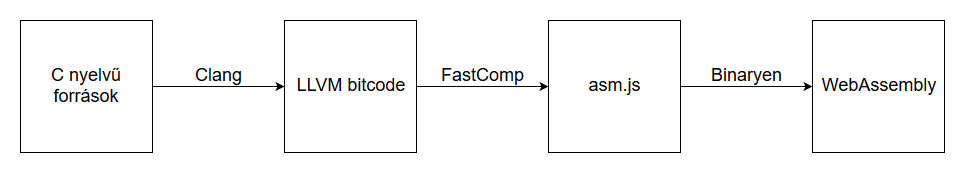
\includegraphics[width=\textwidth]{04-webassembly/emscripten-c-to-wasm.png}
    \caption{C $\rightarrow$ Wasm fordítás Emscriptennel.}
    \label{Figure::WebAssembly::EmscriptenCToWebAssembly}
\end{figure}

A folyamat első lépéseként a Clang fordító az LLVM belső reprezentációjára hozza az eredeti C nyelvű forrásokat. Ez egy könnyen optimalizálható formátum, melyből a FastComp asm.js kimenetet állít elő. Habár ez a köztes lépés nem lenne feltétlenül szükséges, azonban a köztes reprezentációból WebAssemblyt készítő LLVM \textit{backend} még instabilnak tekinthető, így egyelőre érdemesebb ezt az utat választani. A folyamat utolsó lépése a tényleges WebAssembly modul elkészítése, melyről a Binaryen gondoskodik. Természetesen a köztes lépések a felhasználó elől rejtve zajlanak.

Visszatérve a példához, a \texttt{library.c} fordításához szükséges parancsot a \dotref{Listing::WebAssembly::CompileWithEmscripten} kódrészlet tartalmazza. Az \texttt{EXPORTED\_FUNCTIONS} kapcsolóval külön meg kell adnunk a modul kliensei által is látható függvények listáját.

\begin{lstlisting}[language=bash, caption={A \texttt{library.c} fordítása Emscriptennel.}, captionpos=b, label=Listing::WebAssembly::CompileWithEmscripten, numbers=none]
emcc library.c -o library.js \ 
     -s EXPORTED_FUNCTIONS='["_factorial"]' \
     -s EXTRA_EXPORTED_RUNTIME_METHODS='["cwrap"]'
\end{lstlisting}

A futás eredményeként két fájl áll elő: a \texttt{library.wasm} és a \texttt{library.js}. Előbbi a C könyvtárból készült Wasm modul, míg utóbbi egy segédeszközöket tartalmazó JavaScript fájl, mely megkönnyíti a modul JavaScriptből történő felhasználását.

\subsection{Beágyazás HTML-be}

Az elkészült modul HTML kódba történő beágyazását a \dotref{Listing::WebAssembly::EmbeddingHTML} kódrészlet szemlélteti. Ezt egy HTML fájlként elmentve, majd megfelelő (azaz WebAssemblyt támogató) böngészőben megnyitva a „\textit{The factorial of 3 is 6.}” szöveget fogjuk látni.

\begin{lstlisting}[language=HTML, caption={A beágyazó HTML kód.}, captionpos=b, label=Listing::WebAssembly::EmbeddingHTML]
<!doctype html>
<html lang="en">
<head>
    <meta charset="UTF-8">
    <title>Factorial</title>
</head>
<body>
    <p id="result"></p>
    <script type="text/javascript">
        var Module = {
            onRuntimeInitialized() {
                const factorial = Module.cwrap('factorial', 'number', ['number'])

                document.getElementById('result').textContent =
                    `The factorial of 3 is ${factorial(3)}.`
            }
        }
    </script>
    <script async src="library.js"></script>
</body>
</html>
\end{lstlisting}

Ugyan a modul beágyazása a 19. sorban található \texttt{script} elemben történik, ez még csupán a WebAssembly kód feldolgozásáról, validálásáról és JIT vagy AOT fordításáról gondoskodik.

A \texttt{factorial} függvény tényleges futtatásának módját a 12-15. sorokban láthatjuk. Először a 12. sorban a \texttt{cwrap} függvény segítségével egy JavaScript függvényt készítünk az exportált \texttt{factorial} függvényből. A \texttt{cwrap} az exportált függvény neve mellett annak visszatérési típusát, valamint paramétereinek típusát várja. Ezt követően a visszaadott függvény már a szokásos JavaScript függvényekkel azonos módon hívható, amit a 15. sorban láthatunk.

Érdemes még a beágyazó kódban található \texttt{Module} objektumot is megemlíteni (10. sor). Alapesetben az Emscripten által kibocsátott segédkönyvtár egy \texttt{Module} nevű objektumot exportál. Ugyanakkor, ha a beágyazó kód már tartalmaz egy ilyen nevű változót, akkor a segédkönyvtár ezt fogja felhasználni. Az ezen az objektumon definiált \texttt{onRuntimeInitialized} függvény akkor kerül meghívásra, amikor a WebAssembly modul elérhetővé vált, azaz a futtató környezet felkészült a kódvégrehajtásra.
